\subsection{Production of the exclusive Higgs boson}
\label{sec:exclH}
\par With enough shared momentum during a diffractive $pp$ collision, a 125~\GeV\ Standard 
Model Higgs boson (see Section~\ref{sec:higgsSM}) can be created through an exchange of either 
photons or gluons. From the production cross sections shown in Figure~\ref{fig:higgsProdcomp} the 
exchange of gluons is much more preferable than the exchange of photons. The interaction between the 
Higgs boson and the gluons is done through a top quark loop. Since exchange of gluons would 
alter the quantum numbers of the initial and final state protons, another gluon is exchanged 
during the collision to neutralize the overall color. The Feynman diagram in Fig.~\ref{fig:exclH} illustrates 
this process.
 
\begin{figure}[!h]
\centering
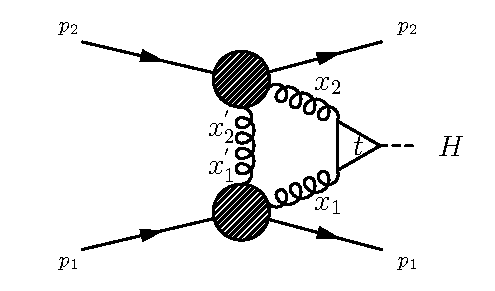
\includegraphics[width=0.8\linewidth]{figures/exclH.pdf}
\caption{Feynman diagram showing the production of the exclusive Higgs boson} 
\label{fig:exclH}
\end{figure}

\par The Khoze-Martin-Ryskin (KMR) model~\cite{Khoze} calculates the cross section for this process, and 
formulates it as 

\begin{equation}
\sigma_{pp(gg)\ra ppH} \propto \hat{\sigma}(gg\ra H)\left ( \int \frac{dQ^2_t}{Q^4_t}f_g(x_1, x_1^{'},Q^2_t)f_g(x_2, x_2^{'},Q^2_t)\right )^2. 
\end{equation}

Here, $\hat{\sigma}(gg\ra H)$ is the cross-section for the gluon fusion process that produces the Higgs boson. This quantity 
can be read directly from Figure~\ref{fig:higgsProdcomp}. The functions $f_g$~\cite{Martin} are the generalized gluon densities
for the finite proton size, that take into account the impact parameter. 
The variables $x_1$ and $x_2$ are the fractions of the momenta carried by the gluons that contribute 
to the production of the Higgs boson, with respect to the momenta of the 
protons $p_1$ and $p_2$. The variables $x_1^{'}$ and $x_2^{'}$ are the fractions 
of the momentum carried by the exchanged third gluon with respect to the momenta of the
protons $p_1$ and $p_2$ as shown in Fig.~\ref{fig:exclH}.
These gluon densities are integrated over the exchanged (third) gluon 
transverse momentum $Q_t$. 

\par For a 125~\GeV\ Standard Model Higgs boson in all decay modes, a total production cross-section 
of 3~fb is predicted when the protons collide at center-of-mass energy $8$~\TeV. The decay modes for the exclusive 
Higgs boson are the same as those discussed in Section~\ref{sec:smHdecay}, and the branching ratios 
are identical to those shown in Figure~\ref{fig:higgsDeccomp}. The analysis discussed in Chapter~\ref{exclH} 
conducts a search for events in which an exclusive Higgs boson is created in $pp$ collision at a center-of-mass 
energy of 8~\TeV.  

